%%
%% Copyright 2007-2020 Elsevier Ltd
%%
%% This file is part of the 'Elsarticle Bundle'.
%% ---------------------------------------------
%% 
%% It may be distributed under the conditions of the LaTeX Project Public
%% License, either version 1.2 of this license or (at your option) any
%% later version.  The latest version of this license is in
%%    http://www.latex-project.org/lppl.txt
%% and version 1.2 or later is part of all distributions of LaTeX
%% version 1999/12/01 or later.
%% 
%% The list of all files belonging to the 'Elsarticle Bundle' is
%% The list of all files belonging to the 'Elsarticle Bundle' is
%% The list of all files belonging to the 'Elsarticle Bundle' is
%% given in the file `manifest.txt'.
%% 
%% Template article for Elsevier's document class `elsarticle'
%% with harvard style bibliographic references

%\documentclass[preprint,12pt,authoryear]{elsarticle}

%% Use the option review to obtain double line spacing
\documentclass[authoryear,11pt]{elsarticle}

%% Use the options 1p,twocolumn; 3p; 3p,twocolumn; 5p; or 5p,twocolumn
%% for a journal layout:
%% \documentclass[final,1p,times,authoryear]{elsarticle}
%% \documentclass[final,1p,times,twocolumn,authoryear]{elsarticle}
%% \documentclass[final,3p,times,authoryear]{elsarticle}
%% \documentclass[final,3p,times,twocolumn,authoryear]{elsarticle}
%% \documentclass[final,5p,times,authoryear]{elsarticle}
%% \documentclass[final,5p,times,twocolumn,authoryear]{elsarticle}

%% For including figures, graphicx.sty has been loaded in
%% elsarticle.cls. If you prefer to use the old commands
%% please give \usepackage{epsfig}

%% The amssymb package provides various useful mathematical symbols

\usepackage[margin=1in]{geometry}
\usepackage{setspace}\linespread{1.4}%

\usepackage{amssymb}
\usepackage{graphicx}
\usepackage{multirow}
\usepackage{amsmath}
\usepackage{dsfont}
\usepackage{afterpage}
\usepackage{hyperref}
\usepackage{xcolor}
\usepackage{tikz}
\usepackage{tabularx}
\usepackage{pdflscape}
\usepackage{algorithm}
\usepackage{algorithmic}
\renewcommand{\algorithmicrequire}{\textbf{Input:}}
\renewcommand{\algorithmicensure}{\textbf{Output:}}
\usepackage{booktabs}
\usepackage[section]{placeins}
\newcommand{\btheta}{\boldsymbol{\theta}}
\newcommand{\bmu}{\boldsymbol{\mu}}
\newcommand{\bSigma}{\boldsymbol{\Sigma}}
\newcommand{\bpsi}{\boldsymbol{\psi}}
\newcommand{\bepsilon}{\boldsymbol{\epsilon}}
\DeclareMathOperator*{\argmax}{arg\,max}
\usetikzlibrary{arrows.meta,positioning,fit,backgrounds}
% Inline TikZ versions of the policy-architecture figures used by
% invman_lostsales.tex. These macros intentionally avoid pre-rendered PDFs.

\colorlet{invblue}{blue!70!black}
\colorlet{invgreen}{green!45!black}
\colorlet{invorange}{orange!75!black}
\colorlet{invred}{red!75!black}
\colorlet{invgray}{black!55}

\tikzset{
  invstage/.style={
    rounded corners=3pt,
    thick,
    align=center,
    inner sep=5pt,
    minimum height=11mm
  },
  invinput/.style={invstage,draw=invgreen!70!black,fill=invgreen!10},
  invmiddle/.style={invstage,draw=invblue!70!black,fill=invblue!8},
  invdecoder/.style={invstage,draw=invorange!80!black,fill=invorange!10},
  invoutput/.style={invstage,draw=invred!70!black,fill=invred!10},
  invflow/.style={-{Latex[length=3.2mm,width=2.2mm]},thick,invblue},
  invsoft/.style={circle,draw=invblue!70!black,fill=invblue!10,thick,
                  minimum size=9mm,inner sep=0pt},
  invleaf/.style={invstage,draw=invgreen!65!black,fill=invgreen!8,
                  minimum width=19mm},
  invbox/.style={draw=invblue!55,dashed,rounded corners=4pt,inner sep=8pt},
  invevsource/.style={invstage,draw=invgreen!70!black,fill=invgreen!10,
                      minimum width=27mm,minimum height=13mm,font=\small},
  invevstock/.style={invstage,draw=invblue!70!black,fill=invblue!8,
                     minimum width=29mm,minimum height=13mm,font=\small},
  invevdemand/.style={invstage,draw=invorange!80!black,fill=invorange!10,
                      minimum width=28mm,minimum height=13mm,font=\small},
  invevlost/.style={invstage,draw=invred!70!black,fill=invred!8,
                    minimum width=28mm,minimum height=13mm,font=\small},
  invmaterial/.style={-{Latex[length=3.4mm,width=2.4mm]},very thick,invblue},
  invrequest/.style={-{Latex[length=3.1mm,width=2.2mm]},semithick,dashed,invgreen!70!black},
  invdemandflow/.style={-{Latex[length=3.4mm,width=2.4mm]},very thick,invorange!85!black},
  invlostflow/.style={-{Latex[length=3.4mm,width=2.4mm]},very thick,dashed,invred},
  invlabel/.style={font=\footnotesize,align=center,fill=white,inner sep=1.5pt},
  invcost/.style={font=\footnotesize,align=center}
}

\newcommand{\PolicyPipelineFigure}{%
\resizebox{0.96\linewidth}{!}{%
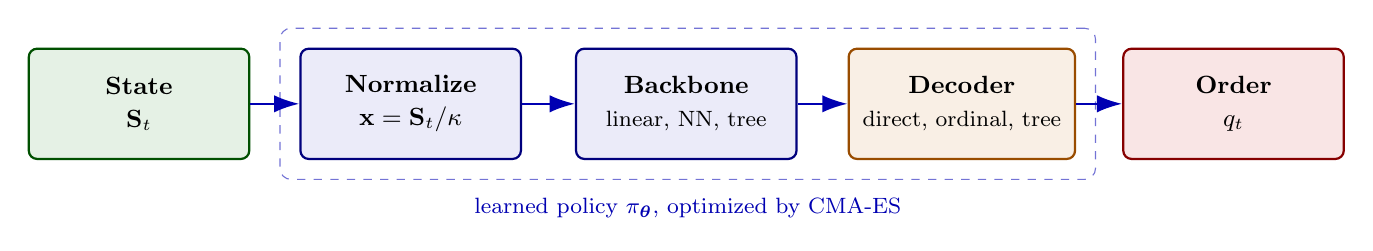
\begin{tikzpicture}[
  x=1cm,y=1cm,
  stagebox/.style={minimum width=28mm,minimum height=14mm,font=\small}
]
  \node[invinput,stagebox] (state) at (0,0)
    {\textbf{State}\\[1pt]$\mathbf S_t$};
  \node[invmiddle,stagebox] (norm) at (3.45,0)
    {\textbf{Normalize}\\[1pt]$\mathbf x=\mathbf S_t/\kappa$};
  \node[invmiddle,stagebox] (backbone) at (6.95,0)
    {\textbf{Backbone}\\[1pt]\footnotesize linear, NN, tree};
  \node[invdecoder,stagebox] (decoder) at (10.45,0)
    {\textbf{Decoder}\\[1pt]\footnotesize direct, ordinal, tree};
  \node[invoutput,stagebox] (action) at (13.9,0)
    {\textbf{Order}\\[1pt]$q_t$};

  \draw[invflow] (state) -- (norm);
  \draw[invflow] (norm) -- (backbone);
  \draw[invflow] (backbone) -- (decoder);
  \draw[invflow] (decoder) -- (action);

  \begin{scope}[on background layer]
    \node[invbox,fit=(norm)(backbone)(decoder),inner sep=7pt] (policy) {};
  \end{scope}
  \node[invblue,fill=white,inner sep=1.5pt,below=5pt of policy.south]
    {\footnotesize learned policy $\pi_{\btheta}$, optimized by CMA-ES};
\end{tikzpicture}}%
}

\newcommand{\LinearPolicyFigure}{%
\resizebox{0.78\linewidth}{!}{%
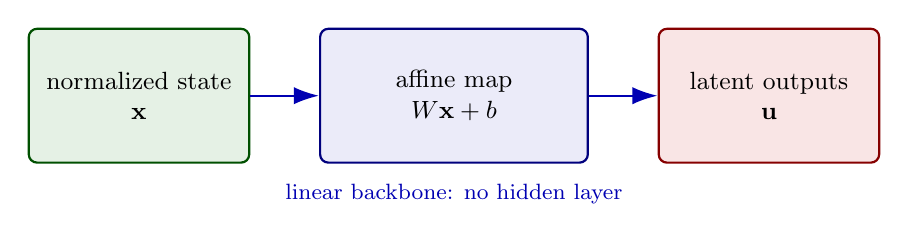
\begin{tikzpicture}[x=1cm,y=1cm]
  \node[invinput,minimum width=28mm,minimum height=17mm,font=\small] (x) at (0,0)
    {normalized state\\$\mathbf x$};
  \node[invmiddle,minimum width=34mm,minimum height=17mm,font=\small] (affine) at (4.0,0)
    {affine map\\$W\mathbf x+b$};
  \node[invoutput,minimum width=28mm,minimum height=17mm,font=\small] (u) at (8.0,0)
    {latent outputs\\$\mathbf u$};

  \draw[invflow] (x) -- (affine);
  \draw[invflow] (affine) -- (u);
  \node[invblue,below=4pt of affine.south,font=\footnotesize,align=center]
    {linear backbone: no hidden layer};
\end{tikzpicture}}%
}

\newcommand{\NeuralPolicyFigure}{%
\resizebox{0.88\linewidth}{!}{%
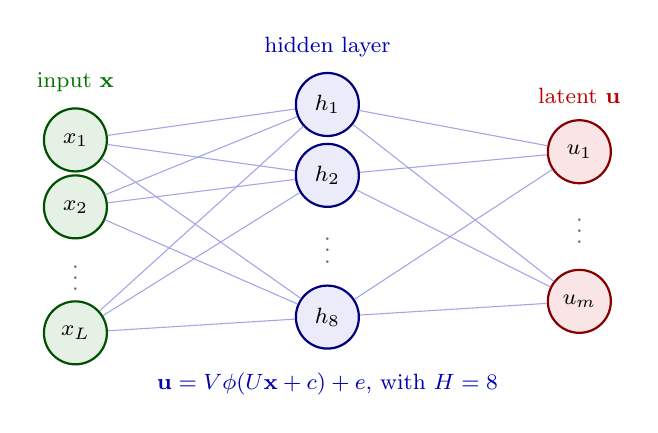
\begin{tikzpicture}[x=1cm,y=1cm]
  \node[invinput,circle,minimum size=8mm,inner sep=0pt,font=\footnotesize] (x1) at (0,1.1) {$x_1$};
  \node[invinput,circle,minimum size=8mm,inner sep=0pt,font=\footnotesize] (x2) at (0,0.25) {$x_2$};
  \node[font=\small,invgray] (xdots) at (0,-0.55) {$\vdots$};
  \node[invinput,circle,minimum size=8mm,inner sep=0pt,font=\footnotesize] (xL) at (0,-1.35) {$x_L$};

  \node[invmiddle,circle,minimum size=8mm,inner sep=0pt,font=\footnotesize] (h1) at (3.2,1.55) {$h_1$};
  \node[invmiddle,circle,minimum size=8mm,inner sep=0pt,font=\footnotesize] (h2) at (3.2,0.65) {$h_2$};
  \node[font=\small,invgray] (hdots) at (3.2,-0.2) {$\vdots$};
  \node[invmiddle,circle,minimum size=8mm,inner sep=0pt,font=\footnotesize] (hH) at (3.2,-1.15) {$h_8$};

  \node[invoutput,circle,minimum size=8mm,inner sep=0pt,font=\footnotesize] (u1) at (6.4,0.95) {$u_1$};
  \node[font=\small,invgray] (udots) at (6.4,0.05) {$\vdots$};
  \node[invoutput,circle,minimum size=8mm,inner sep=0pt,font=\footnotesize] (uM) at (6.4,-0.95) {$u_m$};

  \foreach \i in {x1,x2,xL}{
    \foreach \j in {h1,h2,hH}{
      \draw[invblue!35,thin] (\i) -- (\j);
    }
  }
  \foreach \i in {h1,h2,hH}{
    \foreach \j in {u1,uM}{
      \draw[invblue!35,thin] (\i) -- (\j);
    }
  }

  \node[invgreen,above=2pt of x1.north,font=\footnotesize] {input $\mathbf x$};
  \node[invblue,above=2pt of h1.north,font=\footnotesize] {hidden layer};
  \node[invred,above=2pt of u1.north,font=\footnotesize] {latent $\mathbf u$};
  \node[invblue,below=5pt of hH.south,font=\footnotesize,align=center]
    {$\mathbf u=V\phi(U\mathbf x+c)+e$, with $H=8$};
\end{tikzpicture}}%
}

\newcommand{\DecoderHeadsFigure}{%
\resizebox{\linewidth}{!}{%
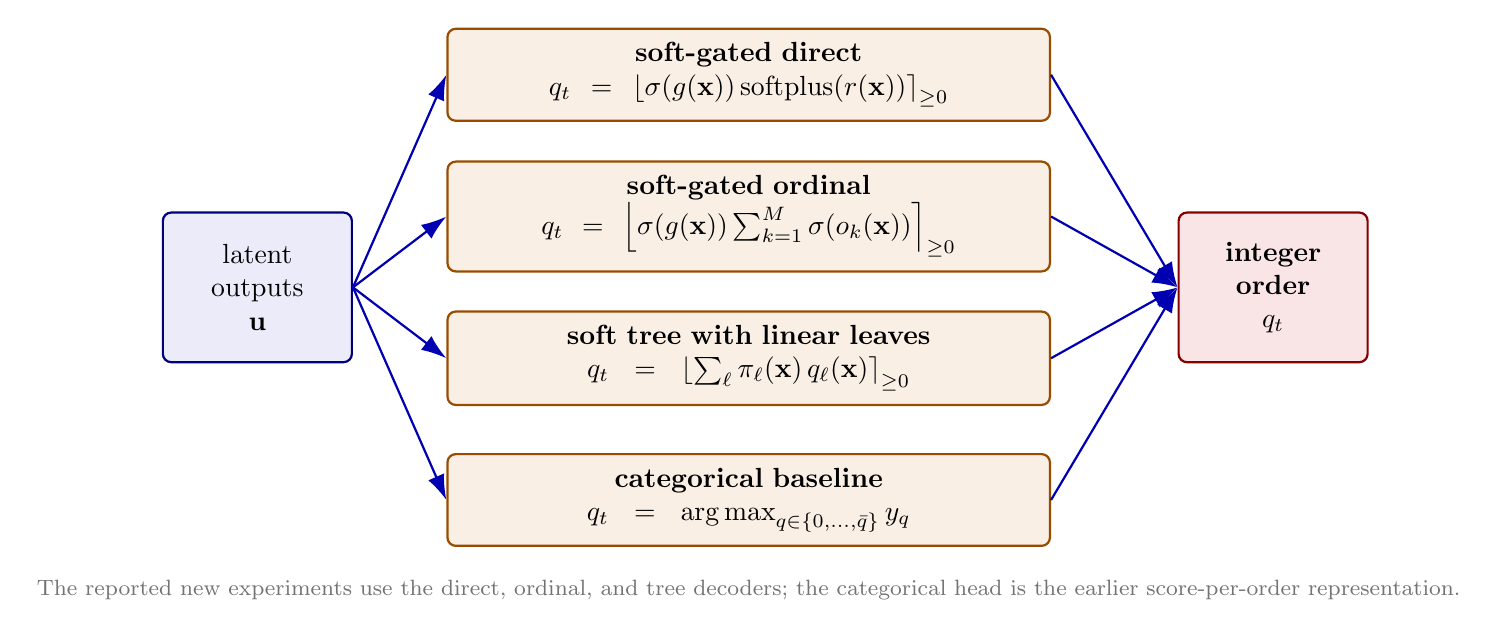
\begin{tikzpicture}[x=1cm,y=1cm]
  \node[invmiddle,minimum width=24mm,minimum height=19mm] (latent) at (0,-2.7)
    {latent\\outputs\\$\mathbf u$};

  \node[invdecoder,anchor=west,text width=73mm] (direct) at (2.4,0)
    {\textbf{soft-gated direct}\\
     $q_t=\left\lfloor\sigma(g(\mathbf x))\,\mathrm{softplus}(r(\mathbf x))\right\rceil_{\ge0}$};
  \node[invdecoder,anchor=west,text width=73mm] (ordinal) at (2.4,-1.8)
    {\textbf{soft-gated ordinal}\\
     $q_t=\left\lfloor\sigma(g(\mathbf x))\sum_{k=1}^{M}\sigma(o_k(\mathbf x))\right\rceil_{\ge0}$};
  \node[invdecoder,anchor=west,text width=73mm] (tree) at (2.4,-3.6)
    {\textbf{soft tree with linear leaves}\\
     $q_t=\left\lfloor\sum_{\ell}\pi_{\ell}(\mathbf x)\,q_{\ell}(\mathbf x)\right\rceil_{\ge0}$};
  \node[invdecoder,anchor=west,text width=73mm] (categorical) at (2.4,-5.4)
    {\textbf{categorical baseline}\\
     $q_t=\argmax_{q\in\{0,\ldots,\bar q\}} y_q$};

  \node[invoutput,minimum width=24mm,minimum height=19mm] (order) at (12.9,-2.7)
    {\textbf{integer}\\\textbf{order}\\$q_t$};

  \foreach \head in {direct,ordinal,tree,categorical}{
    \draw[invflow] (latent.east) -- (\head.west);
    \draw[invflow] (\head.east) -- (order.west);
  }
  \node[invgray,below=3mm of categorical.south,align=center]
    {\footnotesize The reported new experiments use the direct, ordinal, and tree decoders; the categorical head is the earlier score-per-order representation.};
\end{tikzpicture}}%
}

\newcommand{\SoftTreeFigure}{%
\resizebox{0.82\linewidth}{!}{%
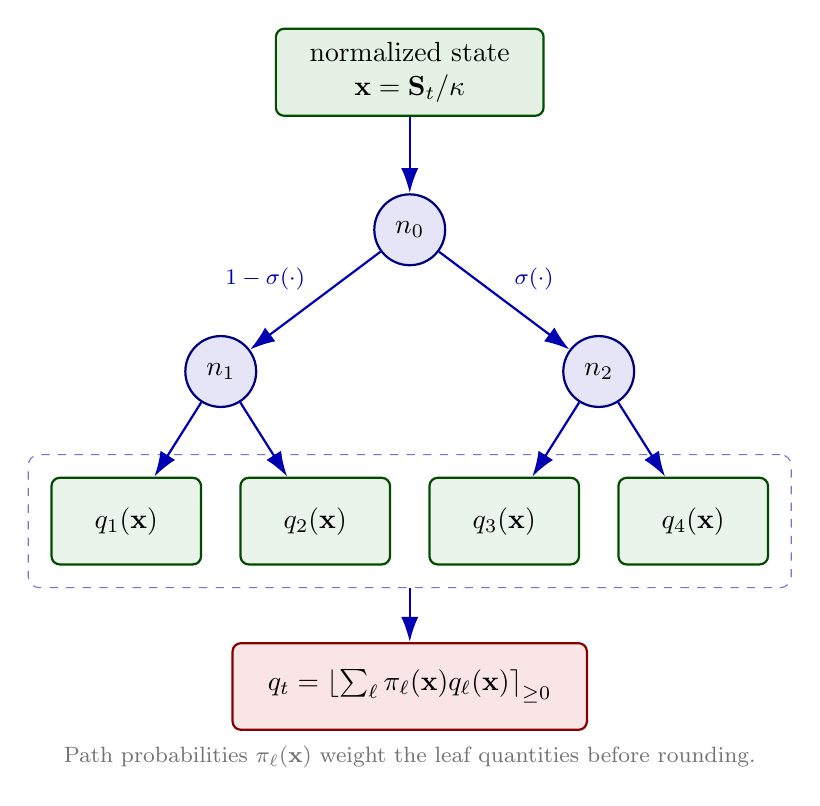
\begin{tikzpicture}[x=1cm,y=1cm]
  \node[invinput,minimum width=34mm] (x) at (0,2.0)
    {normalized state\\$\mathbf x=\mathbf S_t/\kappa$};
  \node[invsoft] (root) at (0,0) {$n_0$};
  \node[invsoft] (left) at (-2.4,-1.8) {$n_1$};
  \node[invsoft] (right) at (2.4,-1.8) {$n_2$};
  \node[invleaf] (l1) at (-3.6,-3.7) {$q_1(\mathbf x)$};
  \node[invleaf] (l2) at (-1.2,-3.7) {$q_2(\mathbf x)$};
  \node[invleaf] (l3) at (1.2,-3.7) {$q_3(\mathbf x)$};
  \node[invleaf] (l4) at (3.6,-3.7) {$q_4(\mathbf x)$};
  \node[invoutput,minimum width=45mm] (out) at (0,-5.8)
    {$q_t=\left\lfloor\sum_{\ell}\pi_{\ell}(\mathbf x)q_{\ell}(\mathbf x)\right\rceil_{\ge0}$};

  \draw[invflow] (x) -- (root);
  \draw[invflow] (root) -- node[above left,font=\footnotesize] {$1-\sigma(\cdot)$} (left);
  \draw[invflow] (root) -- node[above right,font=\footnotesize] {$\sigma(\cdot)$} (right);
  \draw[invflow] (left) -- (l1);
  \draw[invflow] (left) -- (l2);
  \draw[invflow] (right) -- (l3);
  \draw[invflow] (right) -- (l4);

  \begin{scope}[on background layer]
    \node[invbox,fit=(l1)(l2)(l3)(l4)] (leaves) {};
  \end{scope}
  \draw[invflow] (leaves.south) -- (out.north);
  \node[invgray,below=2pt of out.south,align=center]
    {\footnotesize Path probabilities $\pi_{\ell}(\mathbf x)$ weight the leaf quantities before rounding.};
\end{tikzpicture}}%
}

\newcommand{\CMAESLoopFigure}{%
\resizebox{\linewidth}{!}{%
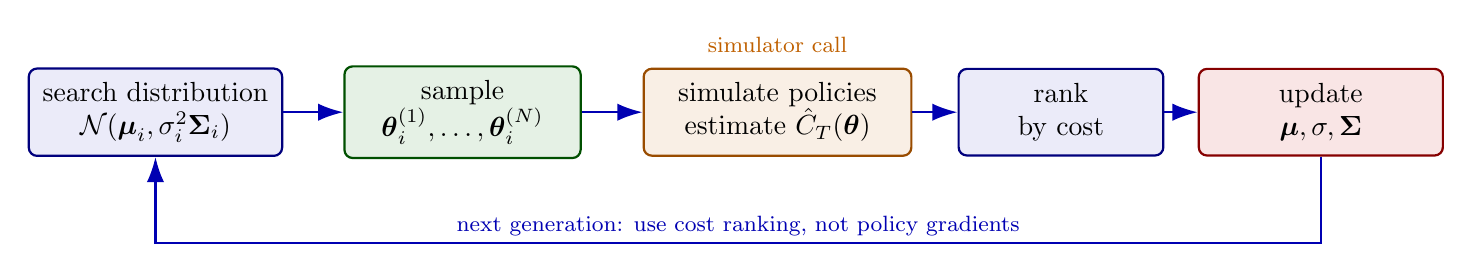
\begin{tikzpicture}[x=1cm,y=1cm]
  \node[invmiddle,minimum width=31mm] (dist) at (0,0)
    {search distribution\\$\mathcal N(\bmu_i,\sigma_i^2\bSigma_i)$};
  \node[invinput,minimum width=30mm] (sample) at (3.9,0)
    {sample\\$\btheta_i^{(1)},\ldots,\btheta_i^{(N)}$};
  \node[invdecoder,minimum width=34mm] (eval) at (7.9,0)
    {simulate policies\\estimate $\hat C_T(\btheta)$};
  \node[invmiddle,minimum width=26mm] (rank) at (11.5,0)
    {rank\\by cost};
  \node[invoutput,minimum width=31mm] (update) at (14.8,0)
    {update\\$\bmu,\sigma,\bSigma$};

  \draw[invflow] (dist) -- (sample);
  \draw[invflow] (sample) -- (eval);
  \draw[invflow] (eval) -- (rank);
  \draw[invflow] (rank) -- (update);
  \draw[invflow] (update.south) -- ++(0,-1.1) -| (dist.south);

  \node[invorange,above=2pt of eval.north] {\footnotesize simulator call};
  \node[invblue] at (7.4,-1.45)
    {\footnotesize next generation: use cost ranking, not policy gradients};
\end{tikzpicture}}%
}

\newcommand{\LostSalesEventFigure}{%
\resizebox{0.98\linewidth}{!}{%
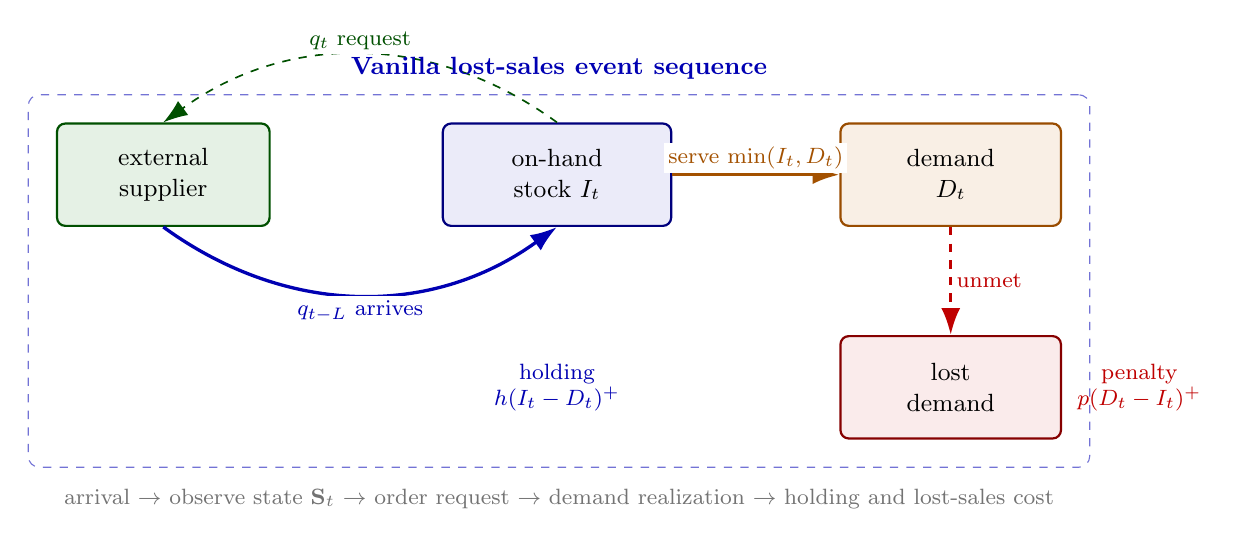
\begin{tikzpicture}[x=1cm,y=1cm]
  \node[invevsource] (sup) at (0,0) {external\\supplier};
  \node[invevstock] (stk) at (5.0,0) {on-hand\\stock $I_t$};
  \node[invevdemand] (dem) at (10.0,0) {demand\\$D_t$};
  \node[invevlost] (lost) at (10.0,-2.7) {lost\\demand};

  \draw[invrequest] (stk.north) to[bend right=36] node[invlabel,above] {$q_t$ request} (sup.north);
  \draw[invmaterial] (sup.south) to[bend right=36] node[invlabel,below] {$q_{t-L}$ arrives} (stk.south);
  \draw[invdemandflow] (stk) -- node[invlabel,above] {serve $\min(I_t,D_t)$} (dem);
  \draw[invlostflow] (dem) -- node[invlabel,right] {unmet} (lost);

  \node[invcost,invblue] at (5.0,-2.7) {holding\\$h(I_t-D_t)^+$};
  \node[invcost,invred,right=2pt of lost.east] {penalty\\$p(D_t-I_t)^+$};

  \begin{scope}[on background layer]
    \node[invbox,fit=(sup)(stk)(dem)(lost),inner sep=10pt] (box) {};
  \end{scope}
  \node[invblue,font=\small\bfseries,above=2pt of box.north]
    {Vanilla lost-sales event sequence};
  \node[invgray,below=4pt of box.south,align=center,font=\footnotesize]
    {arrival $\rightarrow$ observe state $\mathbf S_t$ $\rightarrow$ order request $\rightarrow$ demand realization $\rightarrow$ holding and lost-sales cost};
\end{tikzpicture}}%
}

\newcommand{\FixedCostLostSalesEventFigure}{%
\resizebox{0.98\linewidth}{!}{%
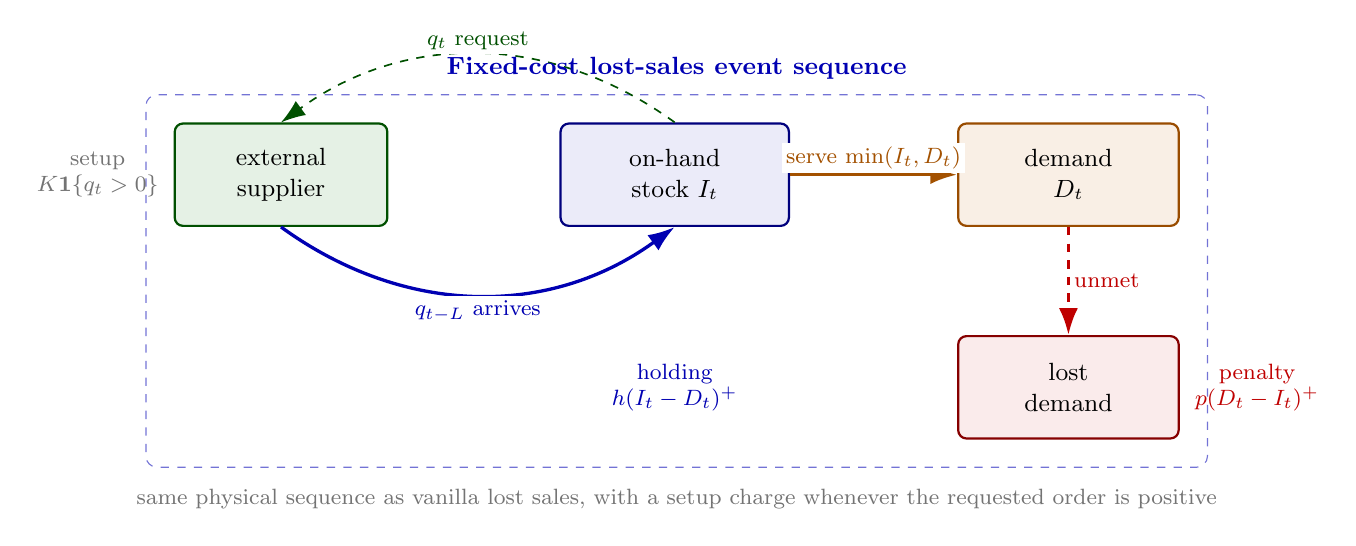
\begin{tikzpicture}[x=1cm,y=1cm]
  \node[invevsource] (sup) at (0,0) {external\\supplier};
  \node[invevstock] (stk) at (5.0,0) {on-hand\\stock $I_t$};
  \node[invevdemand] (dem) at (10.0,0) {demand\\$D_t$};
  \node[invevlost] (lost) at (10.0,-2.7) {lost\\demand};

  \draw[invrequest] (stk.north) to[bend right=36] node[invlabel,above] {$q_t$ request} (sup.north);
  \draw[invmaterial] (sup.south) to[bend right=36] node[invlabel,below] {$q_{t-L}$ arrives} (stk.south);
  \draw[invdemandflow] (stk) -- node[invlabel,above] {serve $\min(I_t,D_t)$} (dem);
  \draw[invlostflow] (dem) -- node[invlabel,right] {unmet} (lost);

  \node[invcost,invblue] at (5.0,-2.7) {holding\\$h(I_t-D_t)^+$};
  \node[invcost,invred,right=2pt of lost.east] {penalty\\$p(D_t-I_t)^+$};
  \node[invcost,invgray,left=2pt of sup.west] {setup\\$K\mathbf{1}\{q_t>0\}$};

  \begin{scope}[on background layer]
    \node[invbox,fit=(sup)(stk)(dem)(lost),inner sep=10pt] (box) {};
  \end{scope}
  \node[invblue,font=\small\bfseries,above=2pt of box.north]
    {Fixed-cost lost-sales event sequence};
  \node[invgray,below=4pt of box.south,align=center,font=\footnotesize]
    {same physical sequence as vanilla lost sales, with a setup charge whenever the requested order is positive};
\end{tikzpicture}}%
}


%% The amsthm package provides extended theorem environments
%% \usepackage{amsthm}

%% The lineno packages adds line numbers. Start line numbering with
%% \begin{linenumbers}, end it with \end{linenumbers}. Or switch it on
%% for the whole article with \linenumbers.
%% \usepackage{lineno}


\newcommand{\hl}{blue}
\begin{document}
\begin{frontmatter}

%% Title, authors and addresses

%% use the tnoteref command within \title for footnotes;
%% use the tnotetext command for theassociated footnote;
%% use the fnref command within \author or \affiliation for footnotes;
%% use the fntext command for theassociated footnote;
%% use the corref command within \author for corresponding author footnotes;
%% use the cortext command for theassociated footnote;
%% use the ead command for the email address,
%% and the form \ead[url] for the home page:
%%
\title{Learning Lost-Sales Inventory Policies with Evolution Strategies:\\ Vanilla and Fixed-Ordering-Cost Settings}

\author{Nima Manaf}
\author{Willem van Jaarsveld}
\author{Rob Basten}
\affiliation{organization={School of Industrial Engineering},%Department and Organization
            addressline={Eindhoven University of Technology},
            city={Eindhoven},
            postcode={5600 MB},
            country={The Netherlands}}

\begin{abstract}
This paper studies compact inventory-control policies for the single-item periodic-review lost-sales problem and its fixed-ordering-cost variant. Exact dynamic programming becomes intractable as lead times grow, while classical heuristics such as myopic, vector base-stock, and $(s,S)$-type policies rely on problem-specific structure. We optimize small policy function approximators directly with Covariance Matrix Adaptation Evolution Strategies (CMA-ES), a gradient-free population-based method that searches over policy parameters using only simulated long-run average costs.

The central design choice is that the action parameterization is part of the policy. Rather than fixing a score for each possible order size, each learned policy maps the state through a compact backbone and then through a policy-owned decoder: soft-gated direct quantities, soft-gated ordinal quantities, or soft decision trees with linear leaves. This distinction is especially important with a fixed ordering cost, where the policy must learn not only how much to order, but whether to order at all.

Across a 24-instance vanilla lost-sales surface, learned policies are instance-best in 22 cases. Across a 48-instance fixed-cost surface, learned policies are instance-best among the available policies in 47 cases. The strongest fixed-cost results come from gated decoders, especially the neural soft-gated ordinal policy, showing that the order/no-order boundary is the key architectural issue. The resulting policies use tens to a few hundred parameters, are trained without per-instance hyperparameter tuning, and remain substantially smaller than typical deep reinforcement learning policies for inventory control.
\end{abstract}

\begin{keyword}
Inventory management \sep Lost sales \sep Fixed ordering cost \sep Evolution strategies \sep CMA-ES \sep Policy optimization
\end{keyword}

\end{frontmatter}

\section{Introduction}
\label{sec:introduction}

Inventory management is a fundamental sequential decision problem in operations management. In each period a controller decides how much to order so as to balance holding costs against shortage costs. Many such problems are naturally formulated as Markov decision processes, but exact dynamic programming is tractable only for small instances because the state space grows rapidly with the lead time. The literature has therefore relied on problem-specific heuristics that exploit structural properties, including base-stock, myopic, vector base-stock, and $(s,S)$-type policies \citep{Zipkin2008OldSystems,Xin2021CappedBaseStock,Bijvank2015ParametricPolicies}.

Deep reinforcement learning (DRL) offers a more generic alternative: represent the ordering policy as a neural network and tune it from simulated experience. Recent work demonstrates that DRL can handle lost-sales and related inventory-control problems \citep{gijsbrechts2022drl,boute2022deep}. The cost of that generality is substantial. DRL implementations often require extensive hyperparameter tuning, value-function or policy-gradient machinery, exploration design, and neural networks with thousands or more parameters. These features make the resulting policies harder to interpret and harder to maintain in practical inventory systems.

We study a different learning recipe for lost-sales inventory control: optimize compact policy approximators directly with Covariance Matrix Adaptation Evolution Strategies (CMA-ES). CMA-ES is a population-based, gradient-free optimizer that adapts a Gaussian search distribution over policy parameters \citep{Hansen2001CompletelyStrategies,Salimans2017EvolutionLearning}. It evaluates policies by their realized simulated cost and updates the search distribution from the best-performing candidates. This avoids action-level credit assignment, value-function approximation, reward shaping, and backpropagation through a simulator.

The paper focuses on two closely related problems. The first is the classical single-item lost-sales problem without fixed ordering costs. The second adds a setup charge whenever a positive order is placed. This fixed-cost variant is not a minor numerical extension: it changes the decision geometry because a good policy must learn an order/no-order boundary. Ordering a little every period can be attractive in the vanilla problem, but is often poor when each positive order triggers a setup cost.

This observation motivates our main methodological choice: the action parameterization is part of the policy. A learned policy first normalizes the inventory state, then applies a compact backbone, and finally uses a decoder that maps latent outputs to a valid integer order. We compare soft-gated direct quantity decoders, soft-gated ordinal quantity decoders, and soft decision trees with linear leaves. The gated decoders explicitly factor the decision into whether to order and how much to order, which is precisely the structural issue introduced by fixed ordering costs.

Our contributions are as follows. First, we provide a focused CMA-ES study for both vanilla and fixed-cost lost-sales inventory control. Second, we show that compact learned policies are competitive with strong lost-sales heuristics on broad benchmark surfaces: learned policies are best in 22 of 24 vanilla instances and in 47 of 48 fixed-cost instances among the available comparators. Third, we show that the decoder matters more than raw network size. Soft trees and linear ordinal decoders are sufficient for many vanilla instances, while gated neural ordinal decoders dominate the fixed-cost setting. Fourth, we retain the practical advantages of compact policies: the learned controllers carry tens to a few hundred parameters and can be evaluated by simple arithmetic at run time.

The remainder of the paper is organized as follows. Section~\ref{sec:literature} reviews learned inventory policies, evolution strategies, and lost-sales heuristics. Section~\ref{sec:policy_representation} describes the policy interface and CMA-ES optimization loop. Section~\ref{sec:lost_sales} formulates the vanilla and fixed-cost lost-sales problems. Section~\ref{sec:experiments} reports the benchmark setup and results. Section~\ref{sec:managerial_insights} discusses practical implications, and Section~\ref{sec:conclusions} concludes. The appendix records the validation anchors for the vanilla and fixed-cost simulators.

\section{Literature}
\label{sec:literature}

The lost-sales inventory problem is a classical benchmark for difficult stochastic inventory control. The system loses unmet demand instead of backordering it, and the pipeline of outstanding orders makes the state dimension grow with the lead time. \citet{Zipkin2008OldSystems} reviews old and new methods for lost-sales systems, and \citet{Xin2021CappedBaseStock} studies the performance of capped base-stock policies. With fixed ordering costs, the relevant heuristic family changes to threshold and batching policies such as $(s,S)$, $(s,nQ)$, and modified $(s,S,q)$ policies \citep{Bijvank2015ParametricPolicies}.

Recent inventory-control research has increasingly adopted DRL and related learned-policy methods. \citet{gijsbrechts2022drl} benchmark A3C on lost sales, dual sourcing, and multi-echelon inventory control; \citet{boute2022deep} provide a broader roadmap for DRL in inventory management; and subsequent work explores larger networks and richer inventory settings \citep{kaynov2024owmr}. These methods demonstrate flexibility, but the typical state-action-reward learning loop requires credit assignment to individual actions and substantial hyperparameter choices.

Evolution strategies provide a simpler policy-search alternative. CMA-ES adapts a full covariance matrix over a Gaussian search distribution and is effective on non-convex, non-smooth, and ill-conditioned optimization landscapes \citep{Hansen2001CompletelyStrategies}. \citet{Salimans2017EvolutionLearning} show that evolution strategies can optimize neural-network policies in large control problems. In inventory control, evolutionary methods have often been used to tune parameters of fixed-form heuristics. Our use is different: we learn the ordering policy itself, but keep the policy compact and structured enough to interpret.

This paper also connects to work on action representations. A neural or linear backbone is only one part of a learned controller; the map from latent outputs to feasible orders can impose or remove useful structure. In lost-sales systems without fixed costs, a plain state-dependent quantity is often enough. With setup costs, the decoder must represent the order/no-order boundary. Our experiments make this action-geometry issue visible by comparing direct, ordinal, and soft-tree decoders under the same CMA-ES optimization loop.

\section{Policy Representation and Optimization}
\label{sec:policy_representation}

\subsection{Policy interface}

A policy is a deterministic map $\pi_{\btheta}$ from the observed state $\mathbf S_t$ to a valid integer order $q_t$. We decompose this map into four steps. First, the raw state is normalized by a fixed scale $\kappa$, giving $\mathbf x=\mathbf S_t/\kappa$. Second, a compact backbone maps $\mathbf x$ to latent outputs $\mathbf u$. Third, a decoder maps those latent outputs to a candidate order quantity. Fourth, the candidate is rounded and projected onto the valid nonnegative integer action set. Figure~\ref{fig:policy_pipeline} shows this interface.

\begin{figure}[!htbp]
\centering
\PolicyPipelineFigure
\caption{Policy interface used in the fixed-cost lost-sales experiments. The policy owns the normalization, backbone, decoder, and projection to a valid action; CMA-ES learns the corresponding parameter vector.}
\label{fig:policy_pipeline}
\end{figure}

We use two backbone classes and one tree mechanism. A linear backbone is a single affine map $u_\theta(\mathbf x)=W\mathbf x+b$. A neural-network backbone is a one-hidden-layer network $u_\theta(\mathbf x)=V\phi(U\mathbf x+c)+e$ with hidden width $H=8$ and SELU activation $\phi$ \citep{Klambauer2017Self}. A soft decision tree routes the normalized state through logistic oblique splits and returns a path-probability mixture of leaf quantities.

\subsection{Decoder heads}

The decoder is the main policy-design choice. Figure~\ref{fig:decoder_heads} summarizes the decoder family.

\begin{figure}[!htbp]
\centering
\DecoderHeadsFigure
\caption{Decoder heads used for lost-sales order quantities. The categorical head is the prior score-per-order representation; the reported new results use soft-gated direct quantities, soft-gated ordinal quantities, and soft trees with linear leaves.}
\label{fig:decoder_heads}
\end{figure}

\paragraph{Soft-gated direct quantity (L-SGD, NN-SGD)}
The backbone emits a gate score $g(\mathbf x)$ and a quantity score $r(\mathbf x)$. The decoder returns
\[
q_t=\left\lfloor \sigma(g(\mathbf x))\,\mathrm{softplus}(r(\mathbf x)) \right\rceil_{\ge0},
\]
where $\sigma$ is the logistic function and $\lfloor\cdot\rceil_{\ge0}$ rounds to the nearest nonnegative integer. The gate controls whether to order; the softplus head controls how much to order.

\paragraph{Soft-gated ordinal quantity (L-SGO, NN-SGO)}
The backbone emits a gate score $g(\mathbf x)$ and $M=20$ ordinal threshold scores $o_1(\mathbf x),\dots,o_M(\mathbf x)$. The decoder returns
\[
q_t=\left\lfloor \sigma(g(\mathbf x))\sum_{k=1}^{M}\sigma(o_k(\mathbf x)) \right\rceil_{\ge0}.
\]
The threshold sum acts as a soft count of units to order. This representation is useful when the policy should batch orders into a few discrete levels.

\paragraph{Soft trees with linear leaves (Tree-1, Tree-2)}
The soft-tree policies use depth-1 or depth-2 oblique splits. Each leaf $\ell$ emits a local softplus-affine quantity $q_\ell(\mathbf x)=\mathrm{softplus}(\alpha_\ell^\top\mathbf x+\beta_\ell)$, and the decoder returns
\[
q_t=\left\lfloor \sum_\ell \pi_\ell(\mathbf x)q_\ell(\mathbf x) \right\rceil_{\ge0},
\]
where $\pi_\ell(\mathbf x)$ is the routing path probability. Figure~\ref{fig:soft_tree} illustrates the depth-2 case.

\begin{figure}[!htbp]
\centering
\SoftTreeFigure
\caption{Depth-2 soft decision tree. The action is the rounded mixture of leaf quantities, weighted by soft routing probabilities.}
\label{fig:soft_tree}
\end{figure}

For an $L=4$ lost-sales state, the direct linear policy has 10 trainable parameters, the direct neural policy has 58, Tree-1 has 15, Tree-2 has 35, L-SGO has 105, and NN-SGO has 229. These policies are much smaller than typical DRL controllers for inventory problems, which often use thousands or more parameters \citep{gijsbrechts2022drl,kaynov2024owmr}.

\subsection{CMA-ES optimization}

CMA-ES samples policy parameters from a multivariate Gaussian search distribution,
\[
\btheta\sim \mathcal{N}(\bmu,\sigma^2\bSigma),
\]
and iterates between sampling candidate policies, evaluating each candidate by simulation, ranking candidates by cost, and updating the mean, step size, and covariance matrix of the search distribution. We use the reference \texttt{pycma} implementation \citep{Hansen2019pycma}. Figure~\ref{fig:cma_loop} shows the loop.

\begin{figure}[!htbp]
\centering
\CMAESLoopFigure
\caption{CMA-ES training loop. Candidate policy parameters are sampled, decoded into policies, evaluated by short rollouts, ranked by simulated cost, and used to update the search distribution.}
\label{fig:cma_loop}
\end{figure}

\begin{algorithm}[!htbp]
\caption{CMA-ES policy optimization}
\label{alg:cmaes-framework}
\begin{algorithmic}[1]
    \STATE \textbf{Input:} population size $N$, initial mean $\bmu_1$, step size $\sigma$, simulator, policy decoder
    \FOR{iteration $i=1,2,\ldots$}
        \STATE Sample $\btheta^{(n)}_i\sim\mathcal{N}(\bmu_i,\sigma_i^2\bSigma_i)$ for $n=1,\dots,N$
        \STATE Evaluate average cost $\hat C_T(\btheta^{(n)}_i)$ by rolling out the decoded policy
        \STATE Update $\bmu_{i+1},\sigma_{i+1},\bSigma_{i+1}$ from the lowest-cost candidates
    \ENDFOR
    \STATE \textbf{Output:} best evaluated policy parameters $\btheta^\star$
\end{algorithmic}
\end{algorithm}

\section{Lost Sales and Fixed-Cost Lost Sales}
\label{sec:lost_sales}

\subsection{Problem formulation}

We study a single-item, periodic-review lost-sales system. Demand and order quantities are integer, demand is stationary, and the controller seeks a stationary policy minimizing long-run average cost. In period $t$, an order placed $L$ periods earlier arrives, the controller observes the post-arrival state, chooses an order $q_t$, demand $D_t$ is realized, and unmet demand is lost.

Let $I_t$ be the on-hand inventory immediately after the period-$t$ arrival. The post-arrival state is
\begin{equation}
    \mathbf S_t=(I_t,q_{t-L+1},\dots,q_{t-1})\in\mathbb{Z}_{\ge0}^{L},
    \label{eq:ls-state}
\end{equation}
where the remaining coordinates are outstanding pipeline orders. The inventory transition is
\begin{equation}
    I_t=(I_{t-1}-D_{t-1})^+ + q_{t-L},
    \label{eq:ls-transition}
\end{equation}
and the full state transition appends the new order to the pipeline:
\begin{equation}
    \mathbf S_{t+1}=\left((I_t-D_t)^+ + q_{t-L+1},q_{t-L+2},\dots,q_{t-1},q_t\right).
    \label{eq:ls-state-transition}
\end{equation}

In the vanilla lost-sales problem, holding cost $h$ is charged per unit left on hand and penalty cost $p$ is charged per unit of lost demand:
\begin{equation}
    c_t = h(I_t-D_t)^+ + p(D_t-I_t)^+.
    \label{eq:ls-cost}
\end{equation}
For policy $\pi_{\btheta}$, the long-run target is
\begin{equation}
    \min_{\btheta}\; \bar C(\btheta),\qquad
    \bar C(\btheta)=\lim_{T\to\infty}\frac{1}{T}\sum_{t=1}^{T}\mathbb{E}[c_t].
    \label{eq:ls-objective}
\end{equation}

The fixed-ordering-cost variant keeps the same state and transition dynamics but adds a setup charge whenever a strictly positive order is placed:
\begin{equation}
    c_t^K = c_t + K\mathbf{1}\{q_t>0\}.
    \label{eq:ls-fixed-cost}
\end{equation}
The objective is again the long-run average cost, now with $c_t^K$ replacing $c_t$. This term makes the order/no-order decision central: a policy that orders small quantities too often pays repeated setup costs, while a policy that waits too long risks lost sales.

\subsection{Policy input and output}

For all lost-sales policies, the input is the state vector in \eqref{eq:ls-state}. The policy divides this vector by $\kappa=20$, applies the selected backbone and decoder, and returns a nonnegative integer order. The maximum ordinal count is $M=20$. These choices are fixed across the benchmark surface; we do not tune the CMA-ES configuration per instance.

To make the decoders concrete, Table~\ref{tab:worked} reports the order returned by each learned decoder on two states of the canonical Poisson-demand instance with $L=4$, $h=1$, $p=4$, and mean demand $5$. The near-empty state $[2,0,0,0]$ triggers larger orders, while the well-stocked state $[8,5,5,5]$ triggers near-replenishment orders.

\begin{table}[!htbp]
\centering
\small
\caption{Worked example: order returned by each learned lost-sales decoder for two states of the Poisson-demand instance with $L=4$, $h=1$, $p=4$, and mean demand $5$. State coordinate $0$ is on-hand inventory; coordinates $1$--$3$ are outstanding pipeline orders.}
\label{tab:worked}
\begin{tabular}{lcc}
\toprule
Decoder & State $[2,0,0,0]$ & State $[8,5,5,5]$ \\
\midrule
Tree-1 & $11$ & $3$ \\
Tree-2 & $14$ & $3$ \\
L-SGD & $12$ & $3$ \\
NN-SGD & $6$ & $4$ \\
L-SGO & $7$ & $4$ \\
NN-SGO & $6$ & $4$ \\
\bottomrule
\end{tabular}
\end{table}

\section{Numerical Experiments}
\label{sec:experiments}

\subsection{Benchmark setup}

The vanilla lost-sales surface uses holding cost $h=1$, mean demand $5$, lead times $L\in\{4,6,8,10\}$, shortage costs $p\in\{4,19\}$, and three demand families: Poisson, Geometric, and positively correlated two-state Markov-modulated Poisson demand (MMPP2$+$). This gives $3\times4\times2=24$ vanilla instances. The fixed-cost surface adds setup costs $K\in\{5,25\}$ to the same instance set, giving $48$ fixed-cost instances.

The vanilla comparators are Myopic-1 (M1), Myopic-2 (M2), and the standard vector base-stock policy (SVBS). The fixed-cost comparators are $(s,S)$, $(s,nQ)$, and modified $(s,S,q)$ policies \citep{Bijvank2015ParametricPolicies}. For fixed-cost policies, the inventory position is $P_t=I_t+\sum_{j=1}^{L-1}q_{t-j}$; threshold policies order only when $P_t$ is sufficiently low.

Training uses CMA-ES with population size $64$ and training horizon $2000$ periods. Evaluation reports long-run average cost over horizon $10^6$ with 10 evaluation seeds. Each cell of the lost-sales surfaces is one CMA-ES optimizer run; robustness is read from the breadth of the 24- and 48-instance grids rather than from selecting the best of multiple optimizer seeds. A dagger in the result tables marks a diverged CMA-ES run, excluded from the comparison.

\subsection{Vanilla lost-sales results}

Table~\ref{tab:results-vanilla-lost-sales} reports the vanilla results. Learned policies are instance-best in 22 of 24 instances. Tree-1 is the most frequent winner with 9 instance wins, followed by L-SGO with 5 wins. The two remaining heuristic wins occur in high-penalty MMPP2$+$ instances at the longest lead times, where the combination of autocorrelated demand and a deep pipeline is hardest for the compact stationary policies.

\begin{table}[!htbp]
\centering
\scriptsize
\setlength{\tabcolsep}{3pt}
\caption{Vanilla lost-sales benchmark: average cost by policy, shortage cost, lead time, and demand family across the reported 24-instance surface.}
\label{tab:results-vanilla-lost-sales}
\resizebox{\textwidth}{!}{%
\begin{tabular}{llrrrrrrrrrrrr}
\toprule
 &  & \multicolumn{3}{c}{Lead time $L=4$} & \multicolumn{3}{c}{Lead time $L=6$} & \multicolumn{3}{c}{Lead time $L=8$} & \multicolumn{3}{c}{Lead time $L=10$} \\
\cmidrule(lr){3-5}\cmidrule(lr){6-8}\cmidrule(lr){9-11}\cmidrule(lr){12-14}
Shortage $p$ & Policy & Pois & Geom & MMPP2$+$ & Pois & Geom & MMPP2$+$ & Pois & Geom & MMPP2$+$ & Pois & Geom & MMPP2$+$ \\
\midrule
$4$ & Optimal & 4.730 & 10.610 &  &  &  &  &  &  &  &  &  &  \\
 & M1 & 5.060 & 11.217 & 9.823 & 5.414 & 11.650 & 11.189 & 5.698 & 11.924 & 12.256 & 5.890 & 12.075 & 13.136 \\
 & M2 & 4.820 & 10.800 & 9.452 & 5.045 & 11.080 & 10.591 & 5.199 & 11.270 & 11.460 & 5.310 & 11.400 & 12.155 \\
 & SVBS & 5.830 & 13.728 & 10.312 & 6.773 & 15.738 & 12.271 & 7.694 & 17.632 & 13.995 & 8.038 & 19.421 & 15.190 \\
 & L-SGD & 4.750 & 10.645 & 8.571 & 4.897 & 10.790 & 9.171 & \textbf{4.974} & \textbf{10.850} & 9.445 & 5.048 & 10.921 & 9.563 \\
 & NN-SGD & 4.774 & 10.687 & 8.565 & 4.900 & 10.791 & 9.643 & 5.033 & 10.983 & 9.674 & 5.066 & 10.993 & 9.697 \\
 & L-SGO & 4.768 & 10.647 & \textbf{8.549} & \textbf{4.893} & 10.823 & \textbf{9.109} & $\dagger$ & 10.884 & \textbf{9.443} & 16.978 & 10.991 & 9.725 \\
 & NN-SGO & 4.786 & 10.692 & 8.577 & 5.064 & 10.799 & 9.183 & 4.978 & $\dagger$ & 9.481 & $\dagger$ & 10.995 & 9.726 \\
 & Tree-1 & \textbf{4.749} & \textbf{10.621} & 8.579 & 4.895 & \textbf{10.776} & 9.159 & 4.975 & 10.857 & 9.445 & \textbf{5.013} & 10.934 & 9.590 \\
 & Tree-2 & 4.750 & 10.670 & 8.595 & 4.936 & 10.820 & 9.302 & 4.977 & 10.892 & 9.446 & 5.067 & \textbf{10.912} & \textbf{9.547} \\
\addlinespace
$19$ & Optimal & 8.890 & 22.950 &  &  &  &  &  &  &  &  &  &  \\
 & M1 & 9.173 & 23.836 & 17.182 & 10.269 & 25.821 & 20.129 & 11.092 & 27.407 & 22.399 & 11.820 & 28.672 & 24.218 \\
 & M2 & 8.953 & 23.280 & 17.644 & 9.831 & 24.930 & 20.474 & 10.511 & 26.210 & 22.552 & 11.090 & 27.270 & \textbf{23.913} \\
 & SVBS & 9.565 & 26.429 & 16.531 & 11.234 & 30.103 & 19.677 & 12.333 & 33.008 & \textbf{22.173} & 13.336 & 35.761 & 24.457 \\
 & L-SGD & 8.932 & \textbf{22.993} & 16.686 & 9.759 & 24.486 & 19.862 & 10.261 & 25.374 & 22.378 & 10.634 & 26.287 & 24.197 \\
 & NN-SGD & \textbf{8.927} & 23.455 & \textbf{16.341} & 10.131 & 24.483 & 19.650 & 10.430 & 25.757 & 22.211 & 10.772 & 26.129 & 24.406 \\
 & L-SGO & 9.003 & 23.240 & 16.491 & 9.794 & 24.370 & \textbf{19.549} & 10.330 & 25.766 & 22.233 & $\dagger$ & 26.171 & 24.345 \\
 & NN-SGO & 8.974 & 23.140 & 16.435 & 9.758 & 24.474 & 19.693 & 10.490 & 25.662 & 22.303 & 10.733 & \textbf{26.037} & 24.357 \\
 & Tree-1 & 8.936 & 23.011 & 16.697 & \textbf{9.711} & \textbf{24.349} & 19.915 & \textbf{10.259} & \textbf{25.209} & 22.339 & \textbf{10.629} & 26.064 & 24.101 \\
 & Tree-2 & 8.941 & 23.043 & 16.683 & 9.720 & 24.430 & 19.864 & 10.272 & 25.382 & 22.301 & 10.698 & 26.174 & 24.193 \\
\bottomrule
\end{tabular}}
\par\medskip\footnotesize Optimal entries are shown only for verified literature optimum anchors; blanks mean no true optimum anchor is available for that expanded instance. $\dagger$: diverged CMA-ES run (excluded). Bold: best reported heuristic or learned policy in the instance column.
\end{table}
\FloatBarrier


On the vanilla surface, the best learned policies are not the largest neural policies. Soft trees and linear ordinal decoders work well because the main task is to produce a state-dependent replenishment quantity. The extra flexibility of neural decoders is not consistently valuable when there is no setup charge.

\subsection{Fixed-cost lost-sales results}

Table~\ref{tab:results-fixed-cost-lost-sales} reports the fixed-cost results. Learned policies are instance-best among the available policies in 47 of 48 instances. NN-SGO is the most frequent winner with 20 instance wins, followed by NN-SGD with 13 wins. The only heuristic instance win is the Geometric instance with $L=4$, $p=4$, and $K=25$, where $(s,nQ)$ and modified $(s,S,q)$ tie.

\begin{table}[!htbp]
\centering
\scriptsize
\setlength{\tabcolsep}{3pt}
\caption{Fixed-ordering-cost lost-sales benchmark: average cost by policy, setup cost, shortage cost, lead time, and demand family across the reported 48-instance surface.}
\label{tab:results-fixed-cost-lost-sales}
\resizebox{\textwidth}{!}{%
\begin{tabular}{lllrrrrrrrrrrrr}
\toprule
 &  &  & \multicolumn{3}{c}{Lead time $L=4$} & \multicolumn{3}{c}{Lead time $L=6$} & \multicolumn{3}{c}{Lead time $L=8$} & \multicolumn{3}{c}{Lead time $L=10$} \\
\cmidrule(lr){4-6}\cmidrule(lr){7-9}\cmidrule(lr){10-12}\cmidrule(lr){13-15}
Setup $K$ & Shortage $p$ & Policy & Pois & Geom & MMPP2$+$ & Pois & Geom & MMPP2$+$ & Pois & Geom & MMPP2$+$ & Pois & Geom & MMPP2$+$ \\
\midrule
$5$ & $4$ & $(s,S)$ & 9.369 & 14.130 & 12.158 & 9.772 & 14.697 &  & 9.965 & 14.839 &  & 10.015 & 15.024 &  \\
 &  & $(s,nQ)$ & 9.211 & 13.968 & 12.113 & 9.385 & 14.177 &  & 9.569 & 14.389 &  & 9.600 & 14.542 &  \\
 &  & $(s,S,q)$ & 9.202 & 13.939 & 12.077 & 9.380 & 14.299 &  & 9.562 & 14.426 &  & 9.826 & 14.524 &  \\
 &  & L-SGD & 8.784 & 14.069 & 12.314 & 9.558 & 13.933 & 12.681 & 9.588 & 14.136 & \textbf{12.722} & 8.934 & 14.023 & 12.818 \\
 &  & NN-SGD & \textbf{8.733} & 13.649 & 13.655 & \textbf{8.871} & \textbf{13.825} & 12.854 & $\dagger$ & 13.910 & 12.940 & 8.933 & \textbf{13.861} & 12.816 \\
 &  & L-SGO & 8.784 & 13.755 & \textbf{11.807} & 9.009 & 13.876 & 12.613 & 8.993 & \textbf{13.847} & 12.751 & 8.943 & 13.942 & 12.808 \\
 &  & NN-SGO & 8.748 & \textbf{13.637} & 11.831 & 8.871 & 13.841 & \textbf{12.363} & 8.909 & 14.144 & 13.010 & 9.153 & 13.866 & 12.817 \\
 &  & Tree-1 & 8.771 & 14.057 & 12.146 & 8.872 & 13.933 & 12.691 & \textbf{8.905} & 14.134 & 12.770 & \textbf{8.931} & 13.871 & \textbf{12.791} \\
 &  & Tree-2 & 8.783 & 13.751 & 11.982 & 9.560 & 13.837 & 12.665 & 8.954 & 13.865 & 12.735 & 8.934 & 14.019 & 12.899 \\
\addlinespace
$5$ & $19$ & $(s,S)$ & 13.889 & 26.888 &  & 14.841 & 28.669 &  & 15.816 & 31.221 &  & 21.667 & 35.693 &  \\
 &  & $(s,nQ)$ & 13.657 & 26.878 &  & 14.694 & 28.872 &  & 15.301 & 29.870 &  & 19.152 & 33.406 &  \\
 &  & $(s,S,q)$ & 13.560 & 26.835 &  & 14.476 & 28.543 &  & 15.618 & 31.067 &  & 21.529 & 35.603 &  \\
 &  & L-SGD & 13.619 & 27.260 & 21.350 & 14.265 & 28.195 & 24.567 & 14.704 & 28.977 & 27.001 & 15.151 & 29.576 & 28.632 \\
 &  & NN-SGD & 13.590 & \textbf{26.531} & \textbf{20.079} & $\dagger$ & 27.941 & 23.306 & 14.770 & $\dagger$ & 25.924 & \textbf{15.030} & 29.822 & \textbf{28.042} \\
 &  & L-SGO & 13.574 & 26.696 & 20.172 & 14.417 & 28.243 & \textbf{23.255} & $\dagger$ & 29.046 & 26.071 & 15.780 & 30.219 & 28.241 \\
 &  & NN-SGO & \textbf{13.475} & 26.602 & 20.208 & \textbf{14.167} & \textbf{27.859} & 23.542 & 14.788 & \textbf{28.936} & \textbf{25.805} & $\dagger$ & 29.879 & 28.079 \\
 &  & Tree-1 & 13.628 & 27.071 & 21.309 & 14.268 & 28.250 & 24.552 & 14.701 & 28.957 & 27.087 & 15.108 & \textbf{29.517} & 28.673 \\
 &  & Tree-2 & 13.613 & 27.078 & 21.325 & 14.260 & 28.177 & 24.642 & \textbf{14.700} & 28.962 & $\dagger$ & 15.044 & 29.615 & 28.847 \\
\addlinespace
$25$ & $4$ & $(s,S)$ & 16.002 & 18.428 & 17.342 & 16.136 & 18.736 &  & 16.331 & 18.925 &  & 16.562 & 19.036 &  \\
 &  & $(s,nQ)$ & 15.840 & \textbf{18.231} & 17.351 & 15.979 & 18.579 &  & 15.837 & 18.649 &  & 16.020 & 18.872 &  \\
 &  & $(s,S,q)$ & 15.877 & \textbf{18.231} & 17.318 & 16.060 & 18.579 &  & 15.806 & 18.648 &  & 16.331 & 18.890 &  \\
 &  & L-SGD & 16.645 & 19.992 & 19.995 & \textbf{15.812} & 19.992 & 19.995 & 16.988 & 19.992 & 19.995 & 17.491 & 19.992 & 18.043 \\
 &  & NN-SGD & \textbf{15.572} & 19.992 & 19.995 & 17.075 & 19.992 & 19.995 & 17.018 & 19.992 & 19.995 & 17.451 & 19.992 & 17.946 \\
 &  & L-SGO & 17.983 & 19.992 & 19.995 & 15.847 & 19.992 & 19.995 & 15.810 & 18.509 & 19.995 & \textbf{15.651} & 19.992 & \textbf{17.786} \\
 &  & NN-SGO & 15.627 & 19.992 & \textbf{17.279} & $\dagger$ & \textbf{18.424} & \textbf{17.840} & \textbf{15.656} & \textbf{18.431} & \textbf{17.753} & 16.271 & \textbf{18.633} & 17.831 \\
 &  & Tree-1 & 20.004 & 19.992 & 19.995 & 18.321 & 19.992 & 19.995 & 19.497 & 19.992 & 19.995 & 17.864 & 19.992 & 19.995 \\
 &  & Tree-2 & 16.203 & 19.992 & 19.995 & 18.167 & 19.992 & 19.995 & 16.632 & 19.992 & 19.995 & 19.710 & 19.992 & 19.995 \\
\addlinespace
$25$ & $19$ & $(s,S)$ & 21.104 & 32.726 &  & 22.073 & 35.015 &  & 25.969 & 38.859 &  & 33.668 & 43.651 &  \\
 &  & $(s,nQ)$ & 21.016 & 32.946 &  & 22.283 & 34.586 &  & 22.664 & 35.812 &  & 25.247 & 38.055 &  \\
 &  & $(s,S,q)$ & 21.016 & 32.772 &  & 22.373 & 35.116 &  & 25.971 & 38.865 &  & 33.995 & 43.652 &  \\
 &  & L-SGD & 21.166 & 32.668 & $\dagger$ & 22.878 & 34.569 & 33.398 & 24.641 & 35.287 & 35.916 & 23.727 & 36.354 & 36.525 \\
 &  & NN-SGD & 20.845 & 32.645 & 27.434 & 21.709 & \textbf{34.021} & \textbf{30.199} & \textbf{22.345} & 35.389 & 32.862 & \textbf{22.772} & $\dagger$ & 34.924 \\
 &  & L-SGO & 21.672 & 32.937 & \textbf{27.386} & 22.447 & 34.256 & 31.004 & 24.816 & 36.025 & 33.133 & 25.213 & 36.400 & 36.811 \\
 &  & NN-SGO & 20.854 & \textbf{32.435} & 27.423 & \textbf{21.598} & 34.185 & 30.495 & 22.752 & \textbf{35.070} & \textbf{32.537} & 23.061 & \textbf{36.005} & \textbf{34.373} \\
 &  & Tree-1 & 21.173 & 32.640 & 28.727 & 21.914 & 35.108 & 33.330 & 22.654 & 35.884 & 35.822 & 23.750 & 36.241 & 37.530 \\
 &  & Tree-2 & \textbf{20.770} & 33.081 & 28.216 & 22.243 & 34.425 & 33.603 & 22.622 & 35.164 & 32.999 & 22.977 & 36.158 & 36.324 \\
\bottomrule
\end{tabular}}
\par\medskip\footnotesize Blank heuristic cells indicate no literature/catalog heuristic value for that MMPP2$+$ instance. $\dagger$: diverged CMA-ES run (excluded). Bold: best reported heuristic or learned policy in the instance column.
\end{table}
\FloatBarrier


The fixed-cost surface is the sharper architectural test. Once every positive order incurs a setup charge, the policy must learn when not to order. The gated decoders explicitly separate whether to order from how much to order, and they dominate the fixed-cost results. The table also exposes a limitation: for $K=25$ and $p=4$, some learned policies collapse to a near never-order policy, visible through repeated costs near $19.992$ or $19.995$. The gated ordinal neural decoder is the most reliable architecture for escaping this collapse.

\section{Managerial Insights and Practical Implementation}
\label{sec:managerial_insights}

The results suggest three practical lessons. First, compact learned policies can compete with strong problem-specific heuristics even in lost-sales systems with long lead times. This matters because lost-sales heuristics require specialized model knowledge, while the CMA-ES loop only needs a simulator and a policy parameterization.

Second, the action decoder should be treated as a design decision. In the vanilla problem, plain quantity decoders and shallow trees are often sufficient. In the fixed-cost problem, the gate is essential because it represents the order/no-order boundary directly. Increasing network size is less important than choosing an action geometry that matches the economic structure of the decision.

Third, these policies are deployable. At run time they reduce to a small number of arithmetic operations on the current inventory and pipeline state. The parameter counts are small enough to inspect, store, and retrain without the organizational overhead associated with large black-box DRL agents.

\section{Conclusions}
\label{sec:conclusions}

This paper studies CMA-ES-trained compact policies for both the classical lost-sales problem and the fixed-ordering-cost variant. The expanded results show that compact policies optimized with CMA-ES are competitive across broad benchmark surfaces: learned policies are best in 22 of 24 vanilla instances and 47 of 48 fixed-cost instances among the available policies.

The main conclusion is architectural. For vanilla lost sales, small trees and linear ordinal decoders often suffice. With fixed ordering costs, gated decoders become decisive because the policy must represent the order/no-order boundary. This finding shifts the paper's emphasis from simply using smaller neural networks to designing the right action parameterization for the inventory economics.

CMA-ES remains attractive because it directly optimizes simulated long-run average cost, requires few hyperparameters, and does not need value-function approximation or reward shaping. Future work should study seed robustness for the few diverged learned cells, investigate restart strategies for high setup-cost regimes, and extend the decoder-design perspective to data-limited and nonstationary lost-sales settings.

\appendix

\section{Environment Validation}
\label{app:validation}

Before relying on the simulators and heuristic stacks for learned-policy comparisons, we validate the implementation against published or reference lost-sales rows. These checks are implementation-fidelity anchors, not learned-policy results.

\subsection{Vanilla lost-sales validation}

For the canonical Poisson instance with $h=1$, $p=4$, $L=4$, and $D_t\sim\mathrm{Poisson}(5)$, the heuristic costs match the reference values used in the lost-sales literature \citep{Zipkin2008OldSystems,Xin2021CappedBaseStock} at the precision reported in Table~\ref{tab:vanilla-lost-sales-validation}.

\begin{table}[!htbp]
\centering
\caption{Published/reference vanilla lost-sales validation example for the canonical Poisson-demand instance.}
\label{tab:vanilla-lost-sales-validation}
\begin{tabular}{lll}
\toprule
Quantity & Published/reference cost & Reproduced cost \\
\midrule
optimal & 4.73 & 4.73 (catalog reference) \\
myopic-1 & 5.06 & 5.0569 \\
myopic-2 & 4.82 & 4.8208 \\
SVBS & 5.83 & 5.8153 \\
\bottomrule
\end{tabular}
\end{table}

\subsection{Fixed-cost lost-sales validation}

For fixed-cost lost sales, we validate against the published example of \citet{Bijvank2015ParametricPolicies}. Their Table~1 reports a Poisson-demand instance with $L=2$, $p=14$, $K=5$, $h=1$, and mean demand $5$. Table~\ref{tab:fixed-cost-validation} shows that the reproduced exact costs match the published values to the table precision.

\begin{table}[!htbp]
\centering
\caption{Published fixed-cost lost-sales validation example from \citet{Bijvank2015ParametricPolicies} and reproduced exact average costs for the reported heuristic parameters.}
\label{tab:fixed-cost-validation}
\begin{tabular}{llll}
\toprule
Policy & Reported parameters & Published cost & Reproduced cost \\
\midrule
optimal & --- & 11.46 & 11.4631 \\
$(s,S)$ & $(17,23)$ & 11.62 & 11.6181 \\
$(s,nQ)$ & $(17,7)$ & 11.56 & 11.5552 \\
modified $(s,S,q)$ & $(17,23,7)$ & 11.50 & 11.4974 \\
\bottomrule
\end{tabular}
\end{table}

\bibliographystyle{elsarticle-harv}
\bibliography{references}

\end{document}
